%%%%%%%%%%%%%%%%%%%%%%%%%%%%%%%%%%%%%%%%
% PDF compatibility code. 

\makeatletter
\newif\ifpdflatex@
\ifx\pdftexversion\@undefined
\pdflatex@false
%\message{Not using pdf}
\else
\pdflatex@true
%\message{Using pdf}
\fi

\newcommand{\latexorpdf}[2]{
  \ifpdflatex@ #2
  \else #1
  \fi
}

\makeatother

#ifdef A4Format
\newcommand{\pformat}{a4paper}
#endif A4Format
#ifdef LetterFormat
\newcommand{\pformat}{letterpaper}
#endif LetterFormat

%%%%%%%%%%%%%%%%%%%%%%%%%%%%%%%%%%%%%%%%

\latexorpdf{
\documentclass[\pformat,12pt,twoside]{jarticle}
}{
% pdftex option is used by graphic[sx],hyperref,toolbox.sty
\documentclass[\pformat,pdftex,12pt]{jarticle}
}

% Ueki change
%\newcommand{\vdmtools}{\textbf{VDMTools}$^{\mathbf{{\textregistered}}}$}
\newcommand{\vdmtools}{\textbf{VDMTools}}
% Ueki change

\newcounter{guideno}
\setcounter{guideno}{1}
\newcommand{\guideline}[1]{%
  \fbox{\parbox{.98\textwidth}{{\bf Guideline \theguideno:} #1
        \addtocounter{guideno}{1}}}}

\usepackage{color}
\usepackage{colortbl}

\newcolumntype{G}{>{\columncolor[gray]{0.8}}p{.9\textwidth}}
\newenvironment{VDMgray}%
{\begin{tabular}{|G|}\hline\small\begin{alltt}}%
{\end{alltt}\normalsize\\
 \hline\end{tabular}}

\setcounter{topnumber}{3}
\def\topfraction{1.0}
\setcounter{bottomnumber}{3}
\def\bottomfraction{1.0}
\setcounter{totalnumber}{3}
\def\textfraction{.1}

\usepackage{times}
\usepackage{longtable,multirow}

% Ueki change start
#ifdef JPN
\AtBeginDvi{\special{pdf:tounicode 90ms-RKSJ-UCS2}}
#endif JPN

\usepackage[dvipdfm,bookmarks=true,bookmarksnumbered=true,colorlinks,plainpages=true]{hyperref}
\usepackage{cite}

\def\seename{$\Rightarrow$}
% Ueki change end

% Ueki delete start
%\latexorpdf{
%\usepackage[plainpages=true,colorlinks,linkcolor=black,citecolor=black,pagecolor=black, urlcolor=black]{hyperref}
%}{
%\usepackage[plainpages=true,colorlinks]{hyperref}
%}
% Ueki delete end

\usepackage{toolbox}
\usepackage{vdmsl-2e}
\usepackage{makeidx}
\usepackage{alltt}
\usepackage{here}

\usepackage{longtable}
\usepackage{ifthen}
% plainpages=false: avoid warning
%   destination with the same identifier already exists
%   but it do not seem to work a the first pages

\usepackage{vpp}

\newcommand{\vdmtoolsver}{v9.0.6}

%\renewcommand{\vdmpp}{{\small VDM}$^{++}$}

\makeatletter
% ------------- TOC manipulation ------------
\def\docglbldepth{1}
%\setcounter{secnumdepth}{\docglbldepth}
%\setcounter{tocdepth}{\docglbldepth}
\def\@pnumwidth{3.0em}
% more space for for >10 subsections
%\def\l@section{\@dottedtocline{1}{1.5em}{3.1em}}
\def\l@subsection{\@dottedtocline{2}{1.5em}{2.8em}}
%\def\l@subsubsection{\@dottedtocline{3}{4.3em}{3.6em}}
%\def\l@paragraph{\@dottedtocline{4}{7.9em}{4.1em}}
%\def\l@subparagraph{\@dottedtocline{5}{10em}{5em}}
\makeatother

\begin{document}

\vdmtoolsmanualcsk{VDM++開発手法ガイドライン}
       {\vdmtoolsver}
       {2016}
       {VDM++}
       {1.0}



% No line numbering
\nolinenumbering
\setindent{outer}{\parindent}
\setindent{inner}{0.0em}

\newcommand{\tab}{\makebox[4em]{}}

\definecolor{color1}{rgb}{0.000,0.000,0.000}
\definecolor{color2}{rgb}{0.000,0.000,1.000}
\definecolor{color3}{rgb}{0.000,1.000,1.000}
\definecolor{color4}{rgb}{0.000,1.000,0.000}
\definecolor{color5}{rgb}{1.000,0.000,1.000}
\definecolor{color6}{gray}{0.5}
%{rgb}{1.000,0.000,0.000}
%\definecolor{not_covered}{gray}{0.5}   %gray for previewing
\definecolor{color7}{rgb}{1.000,1.000,0.000}
\definecolor{color8}{rgb}{1.000,1.000,1.000}
\definecolor{color9}{rgb}{0.000,0.000,0.502}
\definecolor{color10}{rgb}{0.000,0.502,0.502}
\definecolor{color11}{rgb}{0.000,0.502,0.000}
\definecolor{color12}{rgb}{0.502,0.000,0.502}
\definecolor{color13}{rgb}{0.502,0.000,0.000}
\definecolor{color14}{rgb}{0.502,0.502,0.000}
\definecolor{color15}{rgb}{0.502,0.502,0.502}
\definecolor{color16}{gray}{0.5}
%{rgb}{1.000,0.000,0.000}
%\definecolor{not_covered}{gray}{0.5}   %gray for previewing
%\definecolor{color16}{rgb}{0.753,0.753,0.753}

\vfill
\begin{abstract}
オブジェクト指向分析におけるグラフィカルモデルの限界については、広く知られていることである。 視覚化においては優れている一方で、正確かつ明白な記述を行うために十分なものではない。 

本書では、オブジェクト指向形式仕様言語VDM++において、UMLにおけるグラフィカルモデルの利点を形式モデル化や正当性確認への合理的かつ簡易なアプローチに結びつける手法とツールを、\vdmtools\ の機能を借りて明らかにしていく。

\vdmtools\ は VDM++ と UML(Rational Rose) の相互変換を提供している。
これによりUMLのユーザーもまた、不変条件や事前条件および事後条件といった自動的な注釈チェックを用いて、型チェックを行ったり実行可能モデルのテストを行うといった、強化された分析と正当性確認の機能を得ることとなる。

\end{abstract}
\vfill

\newpage

\section{はじめに}

オブジェクト指向モデルにおいては、グラフィカルな視覚化を用いることで、モデル化された``問題''の複雑さに対処して理解を十分深めるための助けが得られる。
グラフィカルな図式を用いると、モデルを抽象化した高水準の概要をつかむことが可能である。これはたとえば、ソフトウェア開発プロセスの早期フェーズでの要求分析に対して、大きな価値となり得る。
また続くフェーズにおいても、再度図式が概要理解を助けてくれるため、コード記述の改良が図れるのである。

分析のためのグラフィカルモデルは、ソフトウェア技術者にとってもプログラミング経験のないクライアントに対しても、両者に適していると言える。
しかしながら、グラフィカルモデルが実際に意味するものに対して、それと異なる認識を人々が持ってしまうことがある。
このような共通理解の欠如が起きる原因はモデルの複雑さにあるとすることはできるが、たとえ小さくてもあるモデルを評価したり検証することは難しいことであるし、さらにグラフィカルモデルに含まれる箱形や矢印がどこまで影響するものなのかを、正確に予見することもまた困難である。

対照的に、実行可能なモデルならばソフトウェア開発過程の早い段階でモデルの有効性が確認されるので、モデル評価の自動化に適している。
グラフィカルなフロントエンドをデザインする高速なプロトタイピング能力と結びつけば、実行可能モデルは手戻り作業の頻度ときつさを大きく削減できるため、生成物を予定通りに予算内で納品することも可能となる。
例えば、技術者はモデルを実行させることで仕様上に即時にフィードバックを得る。
さらにモデルを拡張して、クライアントの問題領域および諸活動と一致させたグラフィカルなフロントエンドとすることで、フロントエンドを介してモデルと直接的な相互作用を行うことができるため、クライアントは諸要求に対する仕様の取り決めを明確に把握できることになる。

本書では、UMLのグラフィカルモデル化の利点をオブジェクト指向形式仕様言語VDM++\footnote{{\small
VDM++ はISO 標準 VDM-SLのオブジェクト指向拡張である。
標準VDM-SL は構造化機構を提供しないが、VDM-SL
ではモジュール群のサポートを行う。  VDM++ は UMLに似たクラスや他の概念のサポートを行う}.}における実行可能モデルの利点と結びつけることで、オブジェクト指向分析および設計を強めていこう、という手法とツールを提供する。
 形式仕様においては、抽象概念を保ちつつも精度を高めることで、モデル化プロセスの改善を図ることができる。
正当性確認プロセスのどの部分においても、精度なしでの自動化は不可能であろう。
またそれらプロセスの、詳細で複雑な実装にではなくむしろ概念上の性質に焦点をあてるためには、抽象化が不可欠なことである。
明白な構造化された方法で要求を述べること、加えて、技術者に親しみやすいツールやテクニック、つまりテストやラピッド・プロトタイピングを用いることで、精度の高いモデルなら自動的に分析され正当性確認がされる。
CSK ではこのアプローチを ``Validated Design through Modelling モデル化を通して正当性確認される設計'' (VDM)と呼び、 \vdmtools\ がこれを裏付けしている。
この文書は、読者が既に一般的なオブジェクト指向ソフトウェア開発にいくらかでも慣れ親しんでいるもの、と仮定している \cite{Meyer88,Shlaer88,Rumbaugh&91}。

\subsection{VDM++ と UML}

大雑把に述べて、同じ方法でソフトウェアの開発を行う会社は2つとない。
たとえ1つの会社内であっても、異なるプロジェクトや人々の間でのソフトウェアプロセスは様々に変化する可能性がある。
%原則として、オブジェクト指向ならばVDM++、構造化ならばVDM-SL、アドホックならばそのどちらかを使い、どのようなソフトウェアプロセスにもこれを改良するアドオンとしてVDMを用いることができる。
オブジェクト指向ならばVDM++、構造化ならばVDM-SL、その他特殊な場合はVDM++またはVDM-SLのどちらかを使い、原則としてどのようなソフトウェアプロセスにもこれを改良するアドオンとしてVDMを用いることができる。
しかしながら本書では、UMLとVDM++がどのように一緒に用いられるかに焦点をあてる。
さらに、要求分析とかシステム設計といったソフトウェア開発の典型的なフェーズのいずれかを区別することなく、どのようにモデルを構築するかに焦点をあてていくこととする。
これはフェーズ間の主な違いというものが、抽象化のレベルにあるからである。
モデルを構築するために基本的なアプローチを行うことと、 \vdmtools\ を用いてこれらのモデルを分析することが、同じになる。

ユーザーにUMLとVDM++の相補的な利点を享受してもらうため、\vdmtools\ のツールセットであるVDM++ ToolboxはRose-VDM++ Link \cite{UMLMan-CSK}\ を提供している。
これにより、UMLモデルとVDM++モデルの間に簡単な移行が用意された。
UMLクラス図は自動的にVDM++の仕様に変換され、逆もまた同様に行えるので、完全な双方向(ラウンドトリップ)エンジニアリング能力を備えたものとなっている。
ユースケースのようなUMLの他の局面も、独立にVDM++モデルのものとして用いることができる。
典型的には、ユースケースはVDM開発に先行することになるであろう。
大雑把に述べてVDM++モデルが実質的な原文であり、そこでしばしば書き落とされたり自然言語であいまいに述べられていた詳細すべては、UMLクラス図の精密版が取り入れる。
それゆえにUMLモデル と VDM++ モデルは相補的なものであって、実際は、同一モデルの2つの見方として捉えることができる。

UMLの最近の版にはOCL(Object Constraint Language) と呼ばれる表記法があるが、これはVDM++と多くの類似点、たとえば事前条件や事後条件、をもつ。
しかしながらVDM++では、 \vdmtools\ を用いてテストを行うという原則に立った正当性確認が可能なので、OCLより好ましいといえる。
OCLでは実行可能な部品を含まないので、これは不可能である。 

本書は、UML、VDM++、あるいは VDM++ Toolboxを完全に紹介しているものではない。
更なる情報を求める場合には、 \cite{Booch&99,LangManPP-CSK,UserManPP-CSK}\ を参考にすることができる。

\subsection{モデルの構築}

モデル構築の方法は、概念の選択のみによるものではない。
モデルの目的は何かが同様に重要不可欠であり、これは分析の種類により決定される。
例えば車を設計する場合、あるモデルの目的は空気力学をテストすることであり、もう1つのモデルの目的はブレーキシステムをテストすることであり、第3のモデルの目的は燃料噴射システムであり、といった具合である。
これらのモデルにおいて、各々を他のモデルと別に抽象化することができる。
たとえば、ブレーキと燃料噴射のシステムモデルでは各々別々の分析が可能だ。
どの詳細を表現し、また分析に関係ないため無視するのかは、抽象化で決定する。
モデル構築上でシステムの複雑さを処理するツールが、抽象化である。 

モデルの目的を設定した後は、以下の手順リストがモデル構築を助けるガイドとなるであろう:

\begin{enumerate}
\item 要求項目を読み取る。
\item 要求項目より機能行動を分析する。
\item 可能性のあるクラスまたはデータ型(通常は名詞) および操作 (通常は動詞)のリストを抽出する。
リスト中の項目に説明を与えることで、用語集の作成を行う。
\item UMLを用いてクラス表示を作図する。
これは属性やクラス間の関連を含むものとなる。
VDM++モデルとしての内部的一貫性をチェックする。
\item 
操作に対するシグニチャを作図する。
VDM++モデルとしての一貫性をチェックする。
\item 要求項目から潜在的な不変条件を決定しそれらを形式化することで、クラス (およびデータ型)の定義を完成する。
\item 事前条件や事後条件そして操作本体を決定することで、必要があれば型定義を修正しながら、操作定義を完成する。
\item テストとラピッド・プロトタイピングを用いて、仕様の正当性確認を行う。
\item 自動コード生成または手動でのコード作成により、モデルを実装する。
\end{enumerate}

ステップ2はUMLから伝統的ユースケースを用いて対処できるであろうし、あるいは構造化から外した少しのVDM定義を行うことで対処できる。
VDM++に初めて挑戦しようとする大部分の読者は、たぶんユースケースの方を用いることと思われるが、もう一方のアプローチについても \cite{CashPoint}\ に記してある。
大まかに述べれば、上記のステップ1から5は、従来通りのオブジェクト指向UML設計にて実装されている部分である。
唯一の違いはステップ4と5において、VDM++を結合することでさらに多くの矛盾を見つけることができるというところにある。
そうとはいえ後で述べるが残りのステップ(6から8)では、システムの統合性を確実のものとするために対処されるべき、大変微妙かつ重要な設計考察の確認を行うことができるのである。

以下の章では、化学プラント向けの簡単なアラームおよび専門家スケジュールシステムに対する要求項目を提示する。
これは本書の残り部分においてモデル化される。
モデル化プロセスは、本書の中では1つのプロセスとして記述されているが、実際の開発においては通常繰り返されるものとなるであろう。
さらに、本書で説明目的に用いる例は大変小さいものであるため、上記リストのステップ2は省いて進めるものとする。

\section{化学プラントの例}

この章では、化学プラントの簡単なアラームシステムに対する要求項目を提示する。
この例は大規模なアラームシステムの部分構成を基に考えられたもので、Fitzgerald と Larsen \cite{Fitzgerald&98b}\ によりVDM-SLの本の中で取り上げられている。
Rose-VDM++ Linkを含めたVDM++ Toolboxの機能を用いて、このシステムモデルを発展させ正当性確認を行っていく。

化学プラントでは、プラント内の状況に反応してアラームを鳴らせるように、数多くのセンサーが装備されている。
アラームが鳴れば、専門家がその場に呼ばれることが必要となる。
専門家は様々なアラームに対処するための様々な資格をもつ。
様々な各々の要求項目は、参照を行うために R1-R8 とラベル付けしてある。

\begin{description}
\item[R1] このプラントのアラームを管理するために、コンピューターベースのシステムが開発されるべきである。
\item[R2] アラームに対処するために4種類の資格が必要とされている。
それらは、電気系資格、機械系資格、生物系資格、化学系資格、である。
\item[R3] システムが稼動している期間では常に、専門家が勤務していなければならない。
\item[R4] 各々の専門家が複数の資格を保有することができる。
\item[R5] システムに報告を行う各々のアラームには、それに関連する資格が1つあり、そのアラームの説明はその専門家であれば理解できるものである。
\item[R6] システムによってアラームが検知された場合は常に、正しい資格を持った専門家を見つけ呼ぶ必要がある。
\item[R7] 専門家は、自分の任務がいつであるかチェックできるシステムデータベースが利用できるべきである。
\item[R8] 任務に就く専門家数の査定が可能でなければならない。
\end{description}

次の章で、これらの要求項目と合致するアラームシステムモデルの開発を始めることとする。

\section{UMLにおけるグラフィカルモデル}

さていよいよ、上記アラームシステムの最初のモデルを開発していこう。
モデルの目的は、アラームを取り扱うために、任務名簿を管理し専門家の呼出しを行うルールを明確にすることである。
UMLで1つモデルを構築し、その一貫性のチェックに \vdmtools\ を使用する。
UML/VDM++組み合わせに特有の手法ガイドラインを強調したい箇所では、短文でのハイライトを行うこととする。

\subsection{用語集の作成}

モデル構築のガイドラインに従って、まず最初に可能性のあるクラスやデータ型のリストを抽出する:

\textbf{潜在的なクラスとデータ型(名詞)}
\begin{itemize}
\item アラーム: 必要資格と警報文
\item プラント
\item 資格 (電気系、機械系、生物系、化学系)
\item 専門家: 保持資格のリスト
\item 時間帯
\item システムおよびシステムデータベース?おそらくはスケジュールの類
\end{itemize}

用語集のこの部分は、Rational RoseといったUMLツールを用いてしばしばクラス図(ダイアグラム)中でモデル化される。
このガイドでは次のステップでなされる。
しかし設計されるべきシステムが大きい場合は、ここに示すようにディレクトリ中のすべての潜在的なクラスと型をシステム立ててリストしておく方が、より安全であるかもしれない。

\textbf{潜在的な操作(動詞)}
\begin{itemize}
\item 専門家を呼出す: アラームが与えられている(必要: アラームオペレーターとシステム)
\item 専門家が任務につく: 任務時間をチェックする(必要: 専門家とシステム)
\item 任務にある専門家の数: 時間帯が与えられている(必要: オペレーター?とシステム)
\end{itemize}

UMLツールを用いることで、用語集のこの部分はしばしばユースケースと同様に記述される。

この簡単なシステムに対して、もっと適した説明もできるであろうが、上記のリストをシステムにおける主概念の用語集として活用していく。

\subsection{クラス表現の作図}

用語集を作成してしまうと、次はクラスと型の違いは何かという説明が必要となる。
純粋なOO アプローチにおいての違いはないのだが、しばしばとても大きなクラス集合を扱うと、クラス数が多いことの複雑さに対処することが困難となる可能性がある、というのが結論である。
VDM++ ではクラスと型の間には1つの違いがあるので、我々のモデルではクラス数削減のためにこれを用いていきたい。
一般的に述べて型は、よくあるOOアプローチにおいてコンテナクラスとして知られるものに相当する。
これらは、このクラスを利用するユーザーが読み書きできる属性を、単にたくさんもっているクラスである。


\guideline{用語集にある名詞は、そのモデルの目的に関して``実質的''機能(読み/書きに加えるもの)をまったく持たないのならば、型としてモデル化されるべきである。}

上記の用語集にある資格は、型としての方がよりよくモデル化される名詞の1例である。
資格は列挙型であるが、ちょうど4つの可能な値をもち明白な機能を持たないからである。
もし我々のモデルの目的が、別々の専門家たちが彼らの資格に基づいて実行できる別々の種類の行為を含むとしたなら、資格は1つのクラスとする方がより自然であったろう。

ここで用語集からアラームと専門家について考察してみよう。
両者とも、例題における物理的世界で現実的な対象物のグループに相当するもので、共存ししかも独立して行動する。
したがってこれら両方を、クラスとしてモデル化していこう:

\begin{description}
\item[アラーム] は属性として \textit{資格} と \textit{警報文}\ をもつクラスである。
警報文は文字列であり、\textit{資格} (図‾\ref{fig:alarm}参照)\ と同様に1つの型と考えることができる。 

\begin{figure}[htbp]
\begin{center}
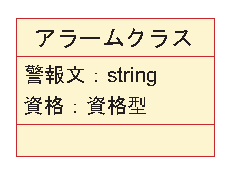
\includegraphics[width=1.833in]{alarm}
\caption{アラームクラス \label{fig:alarm}}
\end{center}
\end{figure}

\item[専門家] は属性として \textit{資格} をもつクラスである。
要求項目では、資格リストがあることと指定している。
単語リストは暗黙にある種の順番を示すものであるが、要求からはこの順番をどのようにすべきかは何もわからない。
このことは我々の``顧客''と共に明らかにする必要があるが、しばらくの間は求められる機能に対して重要性を持つような具体的な順番付けはないと仮定することとする。
図‾\ref{fig:expert}\ に示されている。
\end{description}

\begin{figure}[htbp]
\begin{center}
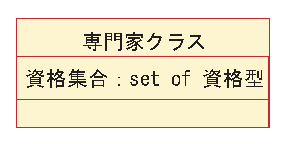
\includegraphics[width=1.833in, height=0.714in]{expert}
\caption{専門家クラス \label{fig:expert}}
\end{center}
\end{figure}

ともかくも、アラームと専門家のスケジュールを関連付ける何らかの結合を行う必要がある。
このような結合に対して、 UML/VDM++ 手法において \textit{厳密な限界}を表すことを可能にするために、他のクラスへの関連を含めたmainクラスの作成を典型として推奨している。


\guideline{異なるクラスとそれらの関連間の厳密な限界がここに表せるような、全システムを象徴する ``main'' クラスを作成する。}


我々の例題中では、 main クラスは \textbf{プラント}\ である。
我々のモデルの目的は、任務スケジュールおよびアラームを処理する専門家の呼出しに関するルールを明確にすること、であることを思い起こそう。
我々はこの目的に焦点をあて、抽象的な展望をモデル化したクラスとしてプラントを選んだ。
それゆえに、 ``プラント'' の2局面: 任務にある専門家の \textit{スケジュール}\ および(登録されている)可能な限りの \textit{アラーム集合}\ の取り集め、が重要である。
まずはアラームについて考えてみよう。
プラントクラスからアラームクラスへの関連が必要であるが、システム内のアラームは複数であり得るため、この関連には多重度を用いる必要がある。
以後この関連を \textit{アラーム集合}\ と呼ぶ(下の図を参照)。 


\guideline{1つの関連が導入された場合は常に、その多重度についての考察が必要で、その関連の利用を望む方向での役割名を与えるべきである。}

次に、様々な時間帯に配置される多くの専門家を包括するスケジュールについて考えてみよう。
各々の時間帯で0人あるいは何人かの専門家が任務につく可能性がある。
このように、時間帯と共に制限が与えられゼロまたはそれ以上の多重度をもつ関連を、我々は用いる必要がある。
この関連を \textit{スケジュール}\ と呼ぶ。


\guideline{ある関連が何かの値にしたがうのならば、その関連に対し制限を与えるものが導入されるべきである。
制限を与えるものの名称は VDM++ 型でなければならない。}


要求項目における時間帯についてはあまり説明されていないため、モデルをこの焦点から多く知る必要はない。
時間帯は``実質的''機能は含まないため、型としてモデル化することができる。

図‾\ref{fig:firstclassdia}\ に示すように、現時点でシステムクラス図は3つのクラスをもつものとして描くことができる。

\begin{figure}[htbp]
\begin{center}
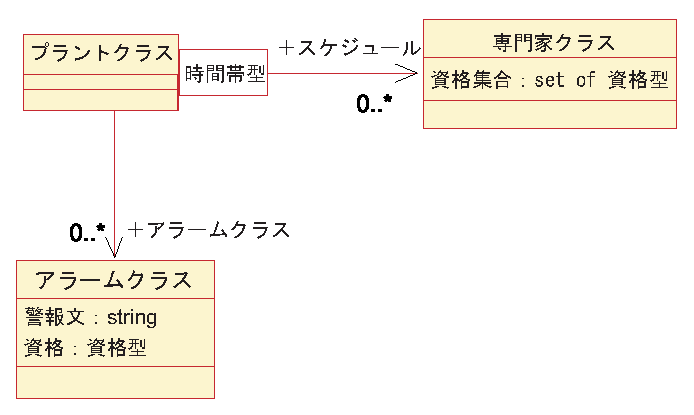
\includegraphics[width=4in]{firstclassdia}
\caption{初期クラス図 \label{fig:firstclassdia}}
\end{center}
\end{figure}

ここで我々は、属性を加えクラス間に関係をもたせるために、 Roseを用いた。
Roseで提供されるテンプレートに従って、属性と型を入力した。
型はVDM++型であり、たとえば、集合型構成子``set of''やクラス名称や他の型識別子といったようなものである。
このすべてをVDM++において直接に、同じように具合よく働かせることができたので、開発者たちは場合によっては、Rose-VDM++ Linkを用いて最初に原文モデルを書きそれからグラフィカルな視覚化を図った方が速いと気づく。

正しいモデルというものは存在しない。
たとえば我々が、このアラームシステムの使用に関連するビジネスプロセスを明示したいと考えたならば、もっと大きなコンピューターシステムの一部としてであったろうし、そしてあそらくはモデルも異なったものとなっていたであろう。
それよりむしろ、どのようにスケジュールが構築されそして保守されるかに焦点をあてたかったのである。

次にはRose-VDM++ Linkを用いて、UML モデルから VDM++スケルトンへ自動的にマッピングする。
これらは以下に含まれる。

\subsubsection*{プラントクラス}

\begin{VDMgray}
--
-- THIS FILE IS AUTOMATICALLY GENERATED!!
--
-- Generated at Mon 09-Aug-99 by the Rose VDM++ Link
--
class プラントクラス

instance variables
 アラーム集合 : set of アラームクラス;
 スケジュール : map 時間帯型 to set of 専門家クラス;

end プラントクラス

\end{VDMgray}

 \emph{スケジュール}\ については、これは UMLでは制限が与えられた関連であるが、VDM++においては写像に変換されていることに注目したい。
1つの写像はテーブルと似ていて、 (定義域において) キーを用いた検索を行い (値域において)それに関連付けられた値を得ることができる。
加えて、ここでのキーは時間帯型であり、値は専門家クラスの集合である。
さらにVDM++の集合型は、\emph{アラーム集合} インスタンス変数におけるのと同様、順をつけない``0以上'' の関連を表すのに用いられることに注目したい。

\subsubsection*{専門家クラス}

\begin{VDMgray}
--
-- THIS FILE IS AUTOMATICALLY GENERATED!!
--
-- Generated at Mon 09-Aug-99 by the Rose VDM++ Link
--
class 専門家クラス

instance variables
 資格集合 : set of 資格型;

end 専門家クラス

\end{VDMgray}

繰り返すが、 VDM++集合型は \emph{資格集合} インスタンス変数に対する``0以上''の多重度とのUML 関連を表すために用いられることに注目したい。

\subsubsection*{アラームクラス}

\begin{VDMgray}
--
-- THIS FILE IS AUTOMATICALLY GENERATED!!
--
-- Generated at Mon 09-Aug-99 by the Rose VDM++ Link
--
class アラームクラス

instance variables
 警報文 : string;
 資格 : 資格型;

end アラームクラス

\end{VDMgray}

 UMLクラスの属性は、UMLの関連と同様に、VDM++ クラスのインスタンス変数になることに注目したい。

\subsubsection*{クラスの型チェック}


\guideline{スケルトンクラスが完成したらすぐ(何らかの機能が導入される前に)、内部的一貫性のチェックのために \vdmtools\ を用いること。}


 \vdmtools\ を用いることで、我々は内部的一貫性の確認のためにモデルの型チェック、つまりすべての識別子がちゃんと定義されているか、を試みることができる。
上記の3つのクラスは、3つの定義されていない識別子: \emph{時間帯型}、\emph{資格型} そして \emph{string} (VDM++のビルトインではない)があるために型が正しいとされない。
したがって、以下の3つの型定義が3つのVDM++クラスのそれぞれに挿入される。

\begin{VDMgray}
class プラントクラス

types
 public 時間帯型 = token;

instance variables 
...

end プラントクラス

\end{VDMgray}

\emph{token}型 は、明確でない値の無限集合を含み、唯一の演算子として等号がある。
時間帯型に対するどのような表現が最終的に実装されるかは現時点では問題にしないため、これを用いる。
ここから抽象化が始まる。
型 \emph{時間帯型} は \texttt{public} に宣言されている必要があるが、 \emph{プラントクラス} の外で利用できなくては困るからである。

\begin{VDMgray}
class 専門家クラス

types
 public 資格型 = \texttt{<}機械\texttt{>} {\textbar} \texttt{<}化学\texttt{>} {\textbar} \texttt{<}生物\texttt{>} {\textbar} \texttt{<}電気\texttt{>};

instance variables 
...
end 専門家クラス

\end{VDMgray}


資格型 は列挙型で、VDM++においては引用型の和集合(垂直バーで表す) として定義されている。
引用型は、それがもつ単一の値と同じ名称をもつが、これは ``\texttt{<}''と``\texttt{>}''記号の中に書かれていなければならない。

\begin{VDMgray}
class アラームクラス

types
 public string = seq of char;

instance variables 
 警報文 : string;
 資格 : 専門家クラス\`{}資格型;

end アラームクラス

\end{VDMgray}


\emph{資格}\ はここで定義されるので、インスタンス変数 \emph{資格型} の前にクラス名称 \emph{専門家クラス} が置かれていることに注目しよう。
Rose-VDM++ Link を用いることで、この変化は図‾\ref{fig:updatedalarm}に示すようにRose UML levelにおいて自動的に更新されている。

\begin{figure}[htbp]
\begin{center}
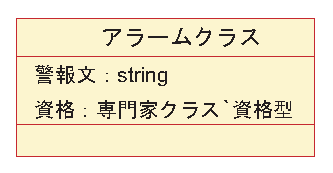
\includegraphics[width=2.120in]{updatedalarm}
\caption{更新されたアラームクラス \label{fig:updatedalarm}}
\end{center}
\end{figure}

UML モデルにおいては、型定義はカウンター部をもたないため、変換されない。
しかしそれらは VDM++モデルファイル内に残され、UML モデル内の更新によって削除(または変更)されることはない。

\subsection{操作に対するシグネチャの作図}

我々はここでUMLの操作シグネチャを追加することにより、開発を続ける。
上記の用語集にリストされている3つの操作は、それらすべて割り当てられたスケジュールに従うものであるため、そのままプラントクラスに属することとなる。 
更新されたプラントクラスのクラス図が、図‾\ref{fig:updatedplant}に示されている。

\begin{figure}[htbp]
\begin{center}
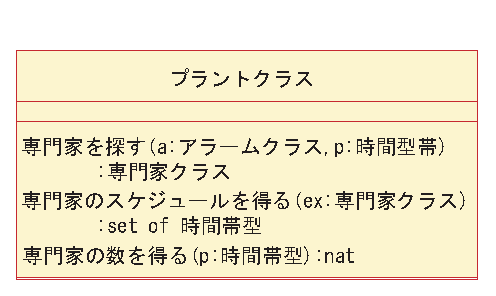
\includegraphics[width=3in]{updatedplant}
\caption{更新されたプラントクラス \label{fig:updatedplant}}
\end{center}
\end{figure}

操作のシグネチャは前方直進型である。
たとえば、 \textit{専門家を探す}\ 操作は入力としてアラームクラスと時間帯型をとり、結果として専門家クラスを返す。

\guideline{パラメーター型と結果型については注意深く考えること。これにより、クラス図の中に欠けていた結合を見つけ出せることが多い。}

更新されたスケルトンのVDM++ クラスは、自動的に生成される。

\begin{VDMgray}
class プラントクラス

types
 public 時間帯型 = token;

instance variables
 アラーム集合 : set of アラームクラス;
 スケジュール : map 時間帯型 to set of 専門家クラス;

operations
 専門家を探す : アラームクラス * 時間帯型 ==\texttt{>} 専門家クラス
 専門家を探す(a, p) ==
   is not yet specified;

 専門家のスケジュールを得る : 専門家クラス ==\texttt{>} set of 時間帯型
 専門家のスケジュールを得る(ex) ==
   is not yet specified;

 専門家の数を得る : 時間帯型 ==\texttt{>} nat
 専門家の数を得る(p) ==
   is not yet specified;

end プラントクラス

\end{VDMgray}


上記のように開発したモデルを構文チェックや型チェックすることは可能だが、様々な正当性確認目的に用いるには精確さに欠けるものである。
我々の次のステップとしては、VDM++を用いてこのモデルにもっと厳密さを与えることだ。
従来よりほとんどのUML開発者は、この段階でストップしてしまっていた。
以下に挙げていくが、最も重要な分析と設計における展開はまだここからなのである。


\section{モデルをより厳密にする}

この段階で、我々のモデルが個々の要求項目を十分に満たすものか、見直すというのもよい考えである。 
明らかに、まだ操作の詳細にわたる考察がなされていないので、\textbf{R6}---\textbf{R8} は完全には網羅できていない。
それ以外は、要求項目\textbf{R3}をいずれでも文書化しなかった場合を除き、要求項目は納得できる程度にはうまく網羅されていたように思える。:

\begin{description}
\item[R3] システムに割り当てられたすべての時間帯で、任務についた専門家がいなければならない。
\end{description}

しかしながら、上記のグラフィック化され型チェックされたVDM++モデルには、以下に述べるが、いくつか更に隠れた仮定と明瞭とはいえない面がある。

モデルを実装する人は典型的に、始めの要求項目から直接行わず、また行うべきでもなく、いくつかコメントを伴った分析や設計のモデルを用いる。
それがモデルの1つの目的ともなっている。
したがってさらに厳密なる抽象化を行えば行うほど、実装を選択するしないにかかわらず、誤った実装を行うというリスクを低減できるのである。

\subsection{不変条件プロパティの追加}

要求項目\textbf{R3}は、VDM++モデルにおいて厳密な方法で形式化することができる。
第一に考えることは、システムにおいて時間帯が割り当てられるとは何を意味するのか?
ということ。これは専門家にとってはスケジュールの中でいつ任務に就くかということであり、つまりインスタンス変数スケジュール定義域において、時間帯型から専門家クラス集合への1つの写像なのである。

\begin{VDMgray}
 forall p in set dom スケジュール \& 
   \textit{時間帯pで任務についている専門家がいる}
\end{VDMgray}

次に考えることは、1つの時間帯に対し専門家が任務についているとは何を意味するのか?ということ。時間帯型と関連する値域の値が、専門家クラスの集合と呼ばれていて、空でないことを意味する。

\begin{VDMgray}
 forall p in set dom スケジュール \& スケジュール(p) \texttt{<}\texttt{>} \{\};
\end{VDMgray}


VDM++においては、この述語は1つの不変条件(\texttt{inv} と略される) として \emph{プラントクラス}のインスタンス変数の部分に加えられている:

\begin{VDMgray}
class プラントクラス
...

instance variables
 アラーム集合 : set of アラームクラス;
 スケジュール : map 時間帯型 to set of 専門家クラス;
 inv 
   forall p in set dom スケジュール \& スケジュール(p) \texttt{<}\texttt{>} \{\};

...
end プラントクラス

\end{VDMgray}


不変条件とは、常にオブジェクトの状態を保持しなければならないという条件である。

\guideline{重要なプロパティあるいは不変条件としての制限は、文書化を試みるべきである。なぜならシステムのある部分で、他の部分では当然気づくであろう何らかの不変条件プロパティの保持を、暗黙に仮定してしまっているかもしれないからである。}

\subsection{操作定義の完成}

次に我々は、操作と関連する条件である事前条件と事後条件のそれぞれについて考える。
事前条件は操作が行う仮定、つまり1つの操作が実行される前にパラメーターやオブジェクト状態の何が保たれなくてはならないのか、の形式化を行う。
事後条件では操作が何をもたらすか、つまり実行が行われた後に何が保持されるか、を述べる。
このように事後条件とは、一方の初期設定のオブジェクト状態とパラメーター値、他方の最終状態と結果値、との間の関係である。
たとえば、操作 \emph{専門家を探す} はアラームクラスと時間帯型を入力として取り込み、アラームクラスを扱う専門家クラスを返す。
では、(事前条件は)任意のアラームクラスや時間帯型を受け入れるのだろうか? 
また、(事後条件は)専門家クラスの何を保持しなければならないのだろうか? 

\texttt{専門家を探す} は以下のシグネチャをもつ:

\begin{VDMgray}
 専門家を探す : アラームクラス * 時間帯型 ==\texttt{>} 専門家クラス
\end{VDMgray}

しかし上記で示されているように、これはどんなアラームクラスも時間帯型も扱えるわけではない。
第一に、任務に就いている専門家がいることを保証するために、時間帯型はスケジュールの中で考えられる必要がある。
アラームはシステム内で登録済みである、つまりインスタンス変数アラーム集合に含まれる限られたものの中にある、という必要性も明らかであろう:

\begin{VDMgray}
 専門家を探す : アラームクラス * 時間帯型 ==\texttt{>} 専門家クラス
 専門家を探す(a, p) ==
   is not yet specified
 pre a in set アラーム集合 and
     p in set dom スケジュール

\end{VDMgray}

さらに、この操作では任務についてしまっている専門家を返すべきではない。
専門家はアラームを扱うための正しい資格を持つべきである。
このことが事後条件において文書化されている。

\begin{VDMgray}
 post let ex = RESULT in
        ex in set スケジュール(p) and
        a.要求される資格を得る() in set ex.資格を得る();
\end{VDMgray}

let式は単純に操作の結果を1つの識別子と結びつける。
最初の連結がこの結果である専門家は任務にあることを述べ、2番目が資格要求に行き着く。
ここで我々は、アクセス操作 \texttt{要求される資格を得る} と \texttt{資格を得る} が各々\texttt{アラームクラス}と\texttt{専門家クラス}に対して定義されていると仮定する。
情報交換を行うために、この種のアクセス操作はOO開発中しばしば定義される必要があるが、定義と言ってもごく簡単である。

この段階で操作の本体を指定する必要はないが、後に操作を実行可能とするために導入されるのである。

ここで与えられた定義では、もし正しい資格をもった複数の専門家が指定の時間帯で任務についている場合に、どの専門家が選ばれるべきかについては述べていない。
要求項目からもっとも望まれる選択は何か知る方法は得られない、だからこそこの暗黙の定義は、後の開発プロセスにおいてこの問題を決定する自由を残してくれているのである。


\guideline{いくつかの選択が可能である場合には、求められている機能を記述する暗黙の方法の利用を試みるべきである。}

ここで、このように正しい資格を持つ専門家を返すことは常に可能なのだろうかと、自問できる。
登録されたアラームに関連し任務につく専門家のスケジュールに制限はない、とする現在のモデルにおいて、確実に返せるとは言えない。
ただし不変条件プロパティを加えることで、この信頼性を導ける。:

\begin{VDMgray}
instance variables
 アラーム集合 : set of アラームクラス;
 スケジュール : map 時間帯型 to set of 専門家クラス;
 inv forall p in set dom スケジュール \& スケジュール(p) \texttt{<}\texttt{>} \{\};
 inv forall a in set アラーム集合 \&
        forall p in set dom スケジュール \&
           exists ex in set スケジュール(p) \&
              a.要求される資格を得る() in set ex.資格を得る();
\end{VDMgray}

新しい不変条件では、システムに登録されたすべてのアラームと時間帯について、そのアラームを操作する正しい資格をもつ専門家がその時間帯内で任務に就いていなければならない、と述べる。
これは、 \texttt{専門家を探す} の記述が意味を持ち実行可能であること、つまり、求められる専門家は常に見つかるということ、を保証する。
VDM++モデルの厳密さのため、システムに求める機能に関連して、我々はこのような詳細にわたり自問自答してきたということに注目して欲しい。
たとえばもしシステムを拡張し、専門家が自ら交替勤務を変更できるよう支援を行うとしたら、上記の不変条件がまた重要となる。
不変条件は、システムに対して支配的な設計要因(パラメーター)となるプロパティを識別するが、それは通常のOOアプローチでは識別されないのである。


\guideline{いくつかの操作が記述されている場合には、不変条件プロパティを追加してプロパティの識別を試みるべきである。}

\texttt{専門家の数を得る} は以下のシグネチャをもつ:

\begin{VDMgray}
 専門家の数を得る : 時間帯型 ==\texttt{>} nat
\end{VDMgray}

これは、与えられた時間帯で任務にある専門家の数を返すものでなければならない。
おそらく我々は時間帯として、スケジュール内の既知のものを求めている。
これは事前条件である。
結果としては、正確にその時間帯で任務に就いている専門家集合の序数となるべきで、
これが操作の本体となる:

\begin{VDMgray}
 専門家の数を得る : 時間帯型 ==\texttt{>} nat
 専門家の数を得る(p) ==
   return card スケジュール(p)
 pre p in set dom スケジュール;

\end{VDMgray}


この場合は事後条件は必要でない。というのはそれは本体をただコピーしただけになってしまうから、公正で高水準な方法で既に記述されているからである。

\texttt{専門家のスケジュールを得る} は以下のシグネチャを持つ:

\begin{VDMgray}
 専門家のスケジュールを得る : 専門家 ==\texttt{>} set of 時間帯型
\end{VDMgray}

専門家には、いつ任務に就いているのか訊ねることができなくてはならないため、この操作に対して事前条件を指定する必要はない。
さらに操作の本体が高水準な方法で自然に記述できるので、事後条件も必ずしも必要でない:

\begin{VDMgray}
 専門家のスケジュールを得る : 専門家 ==\texttt{>} set of 時間帯型
 専門家のスケジュールを得る(ex) ==
   return \{p {\textbar} p in set dom スケジュール \& 
              ex in set スケジュール(p)\};

\end{VDMgray}

この本体は、与えられた専門家が複数の時間帯で任務に就いている場合のように、スケジュール定義域内の時間帯型の集合を返すものである。
厳密で、明瞭で、しかも抽象化されている! 
このような文ならば、プログラム言語中のコード何行かで済むはずである。
Javaではこれが次のようなものとなるであろう: 

\begin{VDMgray}
import java.util.*;

class AlarmClass \{

  Map Schedule;

    Set getExpertSchedule(Integer ex) \{
      TreeSet resset = new TreeSet();
      Set keys = Schedule.keySet();
      Iterator iterator = keys.iterator();

      while(iterator.hasNext()) \{
        Object p = iterator.next();
        if ( ( (Set) Schedule.get(p)).contains(ex))
            resset.add(p);
      \}

      return resset;
   \}
\}

\end{VDMgray}


\guideline{ VDM++における明示的な操作定義は、プログラム言語で書かれたコードと比較して、厳密で明瞭でしかも抽象化したものとなるよう心がけること。}

まとめとして、Rose-VDM++ Linkを用いて、(型チェックされ一貫性のある)VDM++ モデルにおける変更をUMLモデルへマッピングしよう。
結果は次の図の通り:

\begin{figure}[htbp]
\begin{center}
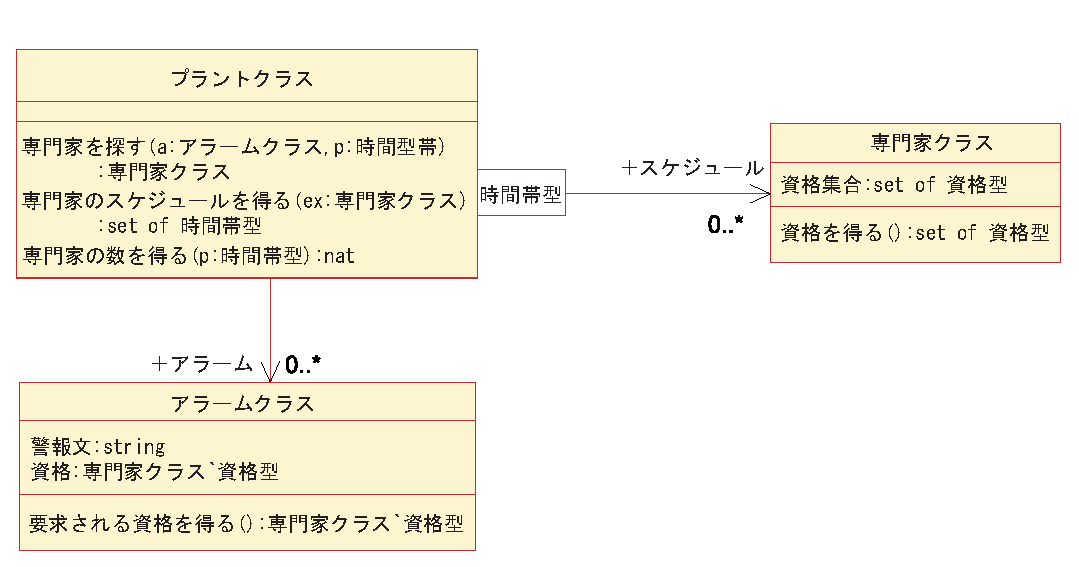
\includegraphics[width=5.5in]{updateddiagram}
\caption{更新されたUMLクラス図 \label{fig:updateddiagram}}
\end{center}
\end{figure}

これはモデルに良い概観を与えているが、要求項目についての詳細な情報はもたない。
 VDM++ モデルは、システム実行に対する本質的な情報をもつ。
このように2つのモデルは、あるいは同一モデルの2つのビューは、相補的である。

\section{VDM++の正当性確認}

前の章で、1つのモデル構成の第一ステップを体験した。
\vdmtools\ の型チェック機能が、モデルの内部的一貫性をチェックするためにどのように用いられるのかを見てきた。
このような機能は役に立つが、すべてのエラーを見つけることができるわけではない。
加えて、顧客が求めたものをモデルが記述していること、また顧客が考えたことを明確にすることが求められたことへの信頼を得るために、正当性確認が用いられる。

本来モデルを検証するには、システムテストとラピッドプロトタイピングのそれぞれをベースとした2つのアプローチがある。
%本質的にモデルの正当性確認には、システムテストとラピッド・プロトタイピングにそれぞれ基盤を置く、2つのアプローチがある。
したがって、\vdmtools\ は他のコード(例えばグラフィカルなフロントエンド)と共に、従来のテスト技術を利用することで、モデルの検証を実現する支援をする。
%したがって \vdmtools\ は、合理的なテスト技術を用いてモデルの正当性確認を行う能力や、他のコード、たとえばグラフィカルなフロントエンド、と共にモデルを実行する能力を支えている。
それ故、VDMToolsのインタープリタでは、それらが実装される前に象徴的に仕様を実行することができる。
%したがって VDM++ Toolbox のインタープリタでは、仕様を実装する前にその仕様の象徴として実行することができる。
実行中は自動的に注釈、つまり不変条件、事前条件、事後条件、のチェックを行う。
何らかの条件が成立しない場合には、ユーザーには違反された条件とどこでその違反が起きたかという具体的な情報が通知される。
%何らかの条件が保持されない場合には、ユーザーには違反された条件とどこでその違反が起きたかという具体的な情報が知らされる。
条件が強ければ強いほど、またテスト範囲が広ければ広いほど、正当性確認の結果としてのモデルの信頼性は高まる。

\subsection{システムテストを用いて自動化された正当性確認}

モデルは伝統的方法でテストされる、したがってこの文書ではテスト理論の詳細に踏み込まない。
しかし、インタープリタの動作に2つのモードが備わっていることには、触れておく価値がある。
モデルの相互作用的なテストが可能で、その場合テスト式がインタープリタに手渡しされすぐに評価がなされる。
他にバッチモードがあり、この場合は潜在的に大きなテストスイート上でインタープリタが自動的に実行される。
このモードでは、実行において統計出力を行うのと同時にモデルの実行されない部分を色分けし、テストカバレッジの提示を行うことができる。

テストを遂行するためには、しばしば、上記に用いている \texttt{要求資格をセットする} や \texttt{警報文をセットする}といった操作のような、異なるインスタンス変数の値を設定する操作を導入する必要が生じる。
さらに、上記で定義された \texttt{専門家を探す}といった操作は、この現在の形式の中での実行は不可能である。
これは我々が陰操作と呼ぶもので、操作本体を持たないからである。
しかしながら、簡単に事後条件を本体に組み入れて操作を実行可能にできる。:

\begin{VDMgray}
  public
  専門家を探す : アラームクラス * 時間帯型 ==\texttt{>} 専門家クラス
  専門家を探す(a, p) ==
    let ex in set スケジュール(p) be st
        a.要求される資格を得る() in set ex.資格を得る()
    in return ex
  pre a in set アラーム集合 and
      p in set dom スケジュール
  post let ex = RESULT in
         ex in set スケジュール(p) and
         a.要求される資格を得る() in set ex.資格を得る();

\end{VDMgray}


これはlet-be-such-that 式と呼ばれる高水準の  VDM++ 式を用いて、``be st'' に続く述語が保持している任意の専門家を選択する。

インタープリタは次のようなコマンドを実行することができる:

\small
\begin{alltt}
  create a1:= new アラームクラス()
  print a1.要求資格をセットする(\texttt{<}機械\texttt{>})
  print a1.警報文をセットする("機械系故障")

\end{alltt}
\normalsize

コマンド \texttt{create} はあるクラスの1つのインスタンスをつくるために用いられる。
コマンド \texttt{print} は、たとえば上記のような手法の起動として、式は評価される。 
各々の行はインタープリタに手動で打ち込むことができるし、あるいはこれらのコマンドを含むスクリプトファイルにすべてのテストシナリオをセットアップすることもできる。
スクリプトファイルはコマンドスクリプトを用いて実行される。
スクリプトファイルは他のスクリプトファイルも同様に呼び込むことができる。
以下のファイルは test1と呼ばれ、インタープリタのウインドウの中で \texttt{script test1}とタイプすることによって実行される。

\small
\begin{alltt}
  init
  script testing/alarm1
  script testing/expert1
  create plant:= new プラントクラス()
  print plant.スケジュールをセットする(\{plant.p1 {\textbar}-\texttt{>} \{ex1\}\})
  print plant.アラームをセットする(\{a1\})
  print plant.専門家のスケジュールを得る(ex1)
  print plant.専門家の数を得る(plant.p1)
  print plant.専門家を探す(a1,plant.p1) 

\end{alltt}
\normalsize

これは2つの他のスクリプトを呼んでいて、ファイル \texttt{alarm1} は新しいアラームオブジェクト \texttt{a1}を定義する:

\small
\begin{alltt}
  create a1:= new アラーム()
  print a1.要求資格をセットする(\texttt{<}機械\texttt{>})
  print a1.警報文をセットする("機械系故障")

\end{alltt}
\normalsize

そしてファイル \texttt{expert1}は新しい専門家クラスオブジェクト \texttt{ex1} を定義する:

\small
\begin{alltt}
  create ex1:= new 専門家クラス()
  print ex1.資格をセットする(\{\texttt{<}機械\texttt{>},\texttt{<}化学\texttt{>}\})

\end{alltt}
\normalsize

テストスクリプトはスケジュールとアラームの集合を更新する。
同時に、不変条件と他のプロパティを自動的にチェックする。

\begin{figure}[ht]
\begin{center}
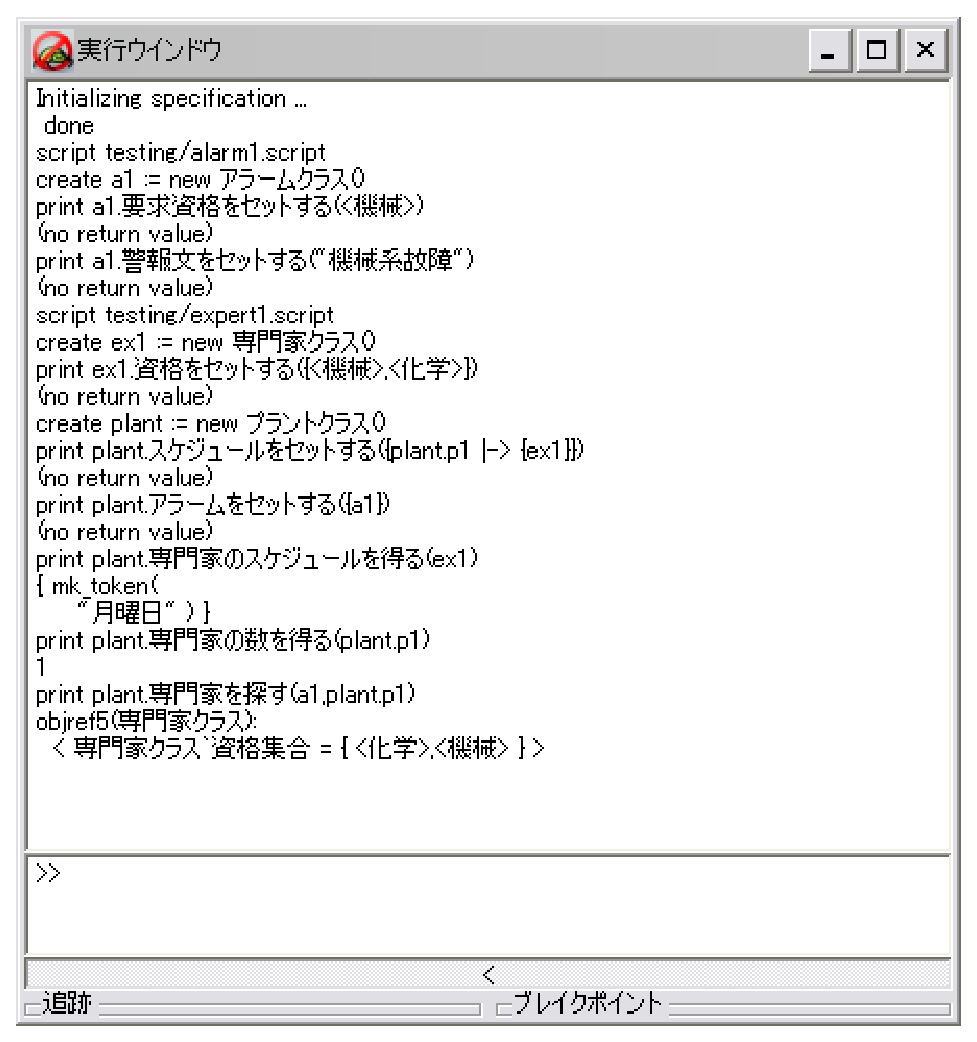
\includegraphics[width=5.546in]{firstscreendump}
\caption{インタープリタの利用 \label{fig:firstscreendump}}
\end{center}
\end{figure}

識別子 \texttt{p1} はtoken定数値で、\texttt{プラントクラス}で定義されている。
テスト中に用いられたクラスのバージョンを、付録Aでみることができる。
上記の図は、図‾\ref{fig:firstscreendump}で表示されたものと同じで、上記  \texttt{test1}スクリプトを実行させた後の Toolbox インタープリタのスクリーンダンプを見せている。

以下のテストスクリプトでは上記 \texttt{test1} を実行し、次に電気系資格を必要とする新しいアラーム \texttt{a2}を追加しようとしている。

\small
\begin{alltt}
  script test1
  script alarm2
  print plant.アラームをセットする(\{a1,a2\})

\end{alltt}
\normalsize

ここに \texttt{alarm2} スクリプトは以下のコマンドを含む:

\small
\begin{alltt}
  create a2:= new アラームクラス()
  print a2.要求資格をセットする(\texttt{<}電気\texttt{>})
  print a2.警報文をセットする("電気系故障")

\end{alltt}
\normalsize

この専門家は電気系資格を持たないことに注意しよう。
そのため 図‾\ref{fig:secondscreendump} に見るスクリーンダンプが示すように、これが不変条件違反で中断する。

\begin{figure}[htb]
\begin{center}
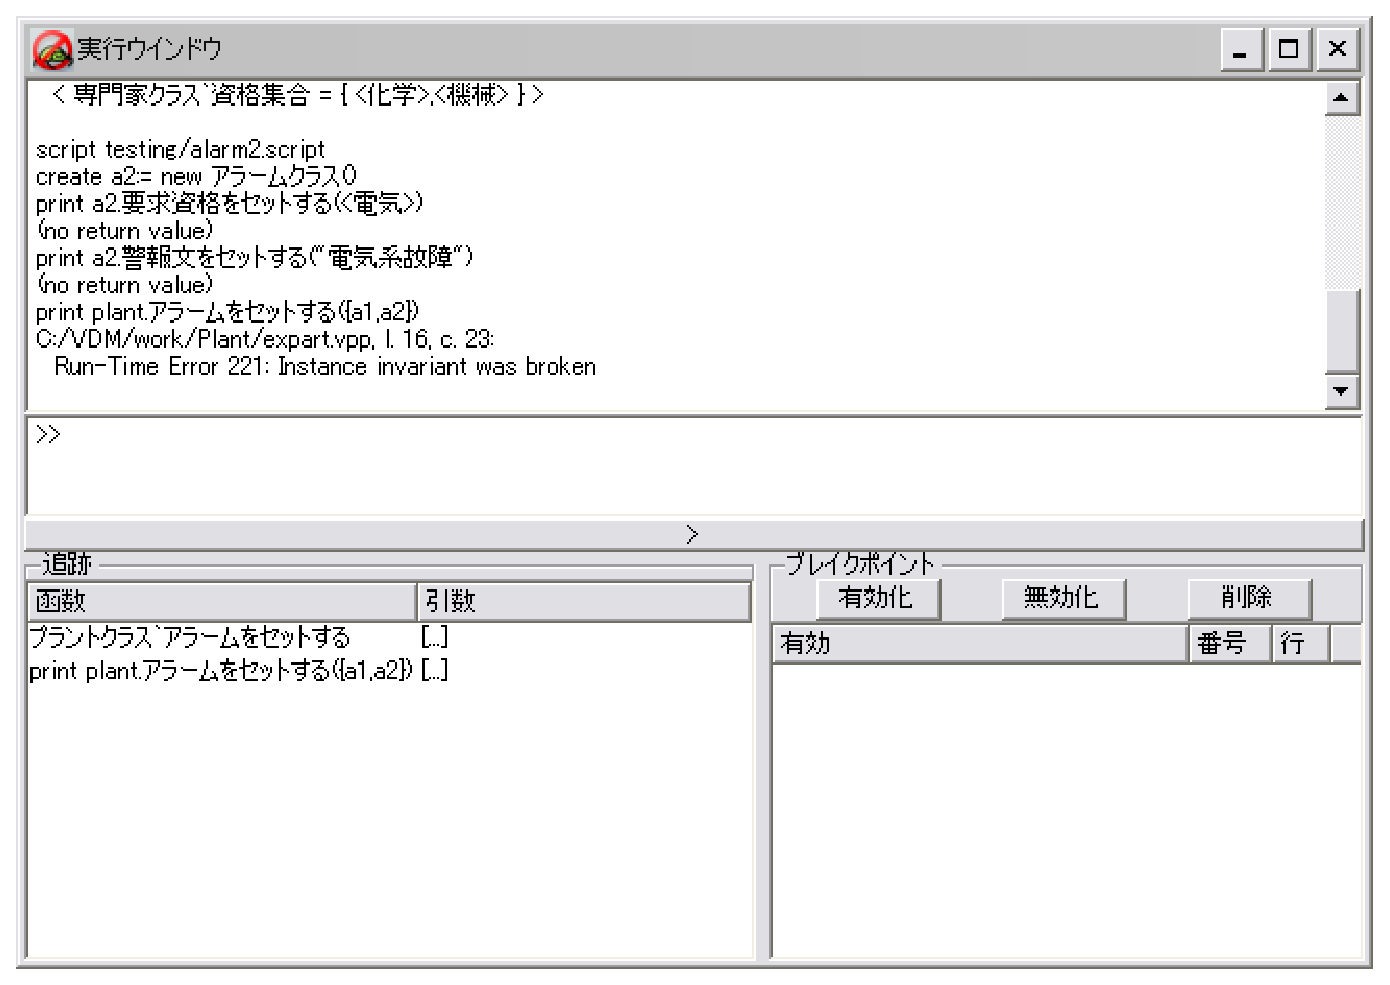
\includegraphics[width=5.546in]{secondscreendump}
\caption{インタープリタにおける不変条件違反の中断 \label{fig:secondscreendump}}
\end{center}
\end{figure}

インタープリタが実行時エラーの具体的な位置情報を提供すること、そしてエラーメッセージが何が誤っているかを示してくれることに注目しよう。
表示画面は仕様ソースの中でどこに問題があったかを表示し、関数トレースが呼出しスタックを、このケースでは一階層のみであるが、与えてくれる。
関数トレース画面で3点をクリックすることで、リストされた操作呼出しの引数が拡張され得る。

インタープリタは、仕様のデバッグにも用いることができる。
関数上にブレークポイントを設定することができるし、その後に相互作用的に実行を1ステップずつ進め、スコープ内の変数を調べることが可能である。

清書機能の一部として、仕様に色を用いてテストカバレッジ情報を清書することが可能である。
%これには Toolboxがコマンドラインから用いられる必要がある。
VDM++ Toolbox はDOSまたはUNIXシェルの中でvppde (VDM++ development environment)をタイプすることで実行される。
このコマンドは様々なオプションを取り、たとえば、``\texttt{-t}''はタイプチェッカーを起動し、 ``\texttt{-i}'' はインタープリタを起動する。
したがって、上記の仕様は次のタイプによって型チェックされる

\small
\begin{alltt}
 vppde -t plant.rtf alarm.rtf expert.rtf
\end{alltt}
\normalsize

コマンドラインインタープリタでは、我々がいわゆるテスト引数ファイルを作成することを要求する。
これには、インタープリタによって評価される式のリストを含めることができる。
以下の \texttt{test1.arg} と呼ばれ上記のテストスクリプトのバージョンで動くファイルを、1つの例としてあげることができる:

\small
\begin{alltt}
 new Test1().run()
\end{alltt}
\normalsize

これは新しいクラス Test1を用いる:

\begin{VDMgray}
class Test1

instance variables
 a1 : アラームクラス;
 ex1 : 専門家クラス;
 plant : プラントクラス;

operations
 public run: () ==\texttt{>} set of プラントクラス\`{}時間帯型 * 専門家クラス
 run() == test1();

 test1: () ==\texttt{>} set of プラントクラス\`{}時間帯型 * 専門家クラス
 test1() ==
   (alarm1();
    expert1();
    plant:= new プラントクラス();
    plant.スケジュールをセットする(\{plant.p1 {\textbar}-\texttt{>} \{ex1\}\});
    plant.アラームをセットする(\{a1\});
    let periods = plant.専門家のスケジュールを得る(ex1),
        expert = plant.専門家を探す(a1,plant.p1)
    in 
      return mk\_(periods,expert));

 alarm1: () ==\texttt{>} ()
 alarm1() ==
   (a1:= new アラームクラス();
    a1.要求資格をセットする(\texttt{<}機械\texttt{>});
    a1.警報文をセットする("機械系故障"));

 expert1: () ==\texttt{>} ()
 expert1() ==
   (ex1:= new 専門家クラス();
    ex1.資格をセットする(\{\texttt{<}機械\texttt{>},\texttt{<}生物\texttt{>}\}))

end Test1

\end{VDMgray}


その後以下のコマンドが実行される: 

\small
\begin{alltt}
  vppde -iDIPQ test1.arg plant.rtf alarm.rtf expert.rtf
\end{alltt}
\normalsize

コマンドラインからテストする間、インタープリタはテストカバレッジ情報を集めることができる。
このためには、最初に以下のようなテストカバレッジファイルを生成する必要がある。

\small
\begin{alltt}
  vppde -p -R vdm.tc plant.rtf alarm.rtf expert.rtf Test1.rtf
\end{alltt}
\normalsize

そしてその後上記の引数ファイルを基盤としたテストケースを実行する

\small
\begin{alltt}
  vppde -iDIPQ -R vdm.tc test1.arg plant.rtf
                                   alarm.rtf expert.rtf Test1.rtf
\end{alltt}
\normalsize

生成された出力ファイルは期待された結果を含むものだ:

\small
\begin{alltt}
  mk\_( \{ mk\_token( 
   "月曜日" ) \},
   objref7(専門家クラス):
   \texttt{<} 専門家クラス\`{}資格集合 = \{ \texttt{<}機械\texttt{>},\texttt{<}生物\texttt{>} \} \texttt{>} )

\end{alltt}
\normalsize

結果であるテストカバレッジ情報は、付録Aにおける清書の仕様で表示されている。

もちろん上記の vppde コマンドはバッチまたは Windows や Unixのシェルスクリプトファイルから呼ぶことができる。
システムテストではこのアプローチが推奨され、Toolbox ユーザーマニュアル \cite{UserManPP-CSK}においてソートの例題に描かれている。

\subsection{ラピッド・プロトタイピングを用いた視覚による正当性確認}

テストはモデルの正当性確認を行うためのすばらしいアプローチであり、技術者たちはテスト技術に精通している。
しかしながら、上記で紹介した比較的低水準のテスト類は、主に技術者に適するもので、 VDM (または UML)やモデルの詳細に親しんでるわけではない顧客や技術外のスタッフおよび管理者に対しては、あまりなじまないものである。
 VDM++ Toolbox は このような聴衆にグラフィカルなフロントエンドを通したモデル提示を行う必要に対して、機能的に働くAPI を準備する。
フロントエンドはこれによりモデルに対するグラフィカルなユーザーインターフェイスとして働くことが可能となり、顧客はGUIを通して、モデルを直接テストすることができる。
アラーム例に対する簡単なフロントエンドの例が図‾\ref{fig:javagui}のようなものである。

\begin{figure}[htbp]
\begin{center}
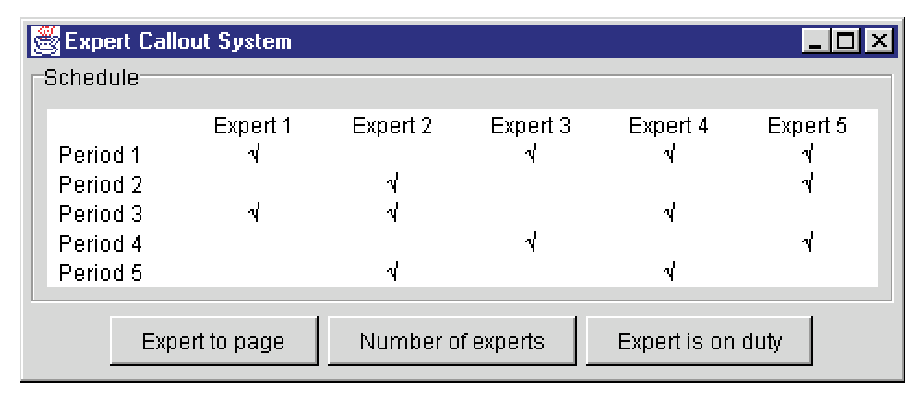
\includegraphics[width=4.999in]{javagui}
\caption{アラームシステムに対するプロトタイプ GUI \label{fig:javagui}}
\end{center}
\end{figure}

明らかにもっと優れたGUIが開発可能であろうが、それは本質ではなく、むしろユーザーはシステムの要求項目に対する開発者の理解をテストするため、簡単にこれを利用できるということの方が本質である。
この方法を利用することで、VDM++モデルはシステムの早期のプロトタイプとして用いられる。
VDM++から独立して、技術者の好みのツールで、フロントエンドをつくりあげることが可能である。
上記のものは Java/Swingで開発されている。

この API はレガシーシステムと共にモデルテストに用いることも可能であり、実際にはプログラム言語から独立した他のコードであって、その一般的性質にしたがうものである。
これは CORBA(the Common Object Request Broker Architecture)を用いているからで、オブジェクトを要求する仲介(ORB)が存在し、何らかの言語で書かれたコードとの通信を許している。
現在すべての主要な言語に対するフリーあるいは商用のORBが複数存在する。
 CORBA がネットワーク基盤の構造であるということは、ネットワーク上に複数配置された外部の顧客が同時並行して1つの VDM++ Toolbox と通信し合えるということも意味する。
そのためこの正当性確認アプローチは、分散モデルに対しても用いることができる。

\section{VDM++モデルのコード生成}

このVDM++モデルはアラームシステムの抽象化モデルであるが、JavaやC++のコード生成、コンパイル、実行、に対応できるほどに十分具体的である。
 VDM++ Toolbox では、直接コンパイル可能で、製品レベルのコードを生成することができるような、自動コード生成を提供する。
一般的に上記のように抽象化されたモデルの場合、コード生成されて顧客に納品されるまでにはもっと多くの手間が必要である。
コード生成を行うためのモデルは一般的には設計や実装指向となるが、特に効率が強く要求される場合などはそうである。
しかし、前の章で紹介したlet-be-such-that式のような高水準の式であっても、JavaやC++でのコード生成、コンパイル、実行は可能である。

実装を行うこの段階で明らかに強力な縮小が行えることに加え、自動コード生成はたくさんの利点をもつ。
原則は、抽象モデルと生成コード間に強い対応性をもつことである。
これがコードとその構成の理解を単純化してくれる。
またこれが、従来モデルのテストに使用されていたテストデータの再利用に向けての可能性を高めている。
もちろん生成されるコードに用いられるアルゴリズムが特定のインスタンスには適当でないこともあるかもしれないが、このような場合は後で手作業で修正できるようなスケルトンコードの生成が可能である。

\section{まとめ}

本書は、VDM++を用いたソフトウェアモデル構築にむけて、いくつかの手法ガイドラインを提示した。
簡単な例である化学プラント向けのアラームシステムに、手法を適用している。
我々は簡潔さを求めるため、提示したモデルでは詳細の多くを省略し抽象化に注意を向けたかった。
しかしながら VDM++ は、もっと具体的でかなり大きいモデルたとえば何百ページにおよぶUMLや何千行ものVDM++に相当するモデルにも、同様によい支援を行うことができる。
今まで述べてきたアプローチでのキーは、UMLとVDM++の結合なので、UMLとVDM++の相補的な利点を最後にまとめることとする。

\subsection{だれがRose-VDM++ Linkを使用すべきか}

以下の2つユーザーグループは、\vdmtools\ とそのRose-VDM++ Linkの恩恵を得られるものと確信する:

\begin{enumerate}
\item
UMLのようなグラフィカルモデル記法をソフトウェア開発において現在適用しているあるいは適用したいと望む人々、またモデルのチェックや正当性確認を改善および自動化したいと望む人々。
これに対する動機付けとしては、彼らのソフトウェアがある程度クリティカルなものかあるいはリスクを削減したいと考えるかであり、そのためVDM技術を用いてできるだけ早くに要求項目を明確にしバグを見つけ、モデルへの早期の高い信頼を得たいと望むからである。

\item
VDM++のようなオブジェクト指向形式仕様言語を開発に適用しているあるいは適用したいと望む人々、また文書化目的でグラフィカルな視覚化能力を処理したりあるいはモデルのチェックや正当性確認を改善および自動化したいと望む人々。
\end{enumerate}


両グループともたぶん多かれ少なかれ同じやり方で、リンクを用いることになるであろう。
第一のグループはUMLの方でより多く、一方で第二のグループはVDM++の方でより多くモデル化を行おうとするかもしれないが、 リンクのラウンドトリップエンジニアリングが両グループにとっての中枢となるはずである。
そのため、問題の全体像を把握するためにはグラフィカルな表記法がより優れていることから、ユーザーはUMLレベルのモデル化からスタートすることで利益を得ることとなる。 
一旦モデルが比較的安定した状態に到達すれば、VDM++に変換しそこで分析を続けるとか、あるいは2つの表記法の間で必要に応じて行ったりきたりを切り替えることが、適切に行えるようになる。

\subsection{UMLにおけるグラフィカルなモデル化}

我々は UML と Rose は次のことにより適していると考える
\begin{itemize}
\item
あるソフトウェアシステムのオブジェクト指向モデルの最初の作図を行う(ある程度は書面で補う)こと
\item
クラス名、属性や操作の名称、操作のシグネチャ、そしてクラス(継承、関連、役割、名称、他)間の関係のようなモデルの視覚的な面を、グラフィカルに定義すること
\item
例えば異なった図表示を通しての、モデルの視覚的で効率的なプレゼンテーション
\item
そして、抽象化された高水準のソフトウェアモデルの様相
\end{itemize}


このようなUMLとRoseの仕様例は本書で示されている。

\subsection{\vdmtools を使用したモデルの分析}

VDM++ と \vdmtools は、次の点においてより適したものであることを確信している

\begin{itemize}
\item
求められている機能の詳細な記述を行うこと、たとえばインスタンス変数におけるVDM++不変条件や、操作における事前条件や事後条件のように、要求項目のプロパティを形式化することによってである、 
\item
型チェックを用いてモデルの内部的一貫性をチェックすること、たとえば宣言の中で操作のシグネチャや型(UMLにおいては属性や関連)をチェックするというようなこと、
\item
どのような操作を行うべきかといったモデルの具体的様相を定義しチェックすること、通常ならばツールなどでチェックされ得ない自然言語で表現されるようなことをである、
\item
文書化されたプロパティを一貫してチェックする一方、モデルの実行とテストに基づくシステマチックで反復可能なチェックプロセスを通し、モデルに対する信頼を得ること、そして、
\item
グラフィカルなフロントエンド、あるいは新しいコンポーネントが具体的に記されている既存のソフトウェアと共に、モデルが実行される場所でラピッド・プロトタイピングを行うこと。
\end{itemize}


SAFERモデルのあるバージョンを分析するためのVDM技術の効果的利用が、論文 \cite{Agerholm&97c,Agerholm&99}に記述されている。
SAFER というのは、宇宙飛行士のための、修理を行うために宇宙船外に出るときに身に着けるバックパック部材である。
安全面でかつセキュリティ面で重要な領域にあるVDM技術についての他の論文 \cite{Agerholm&98a,Larsen&96a}、もまた興味を引くものである。

\bibliographystyle{iptes}

\bibliography{ifad}

\newpage
\appendix
\section{UMLモデルとVDM++モデル}


この付録は、化学プラントの例におけるモデルを清書したVDM++クラスにテストクラスを加えて、リストする。
各々のクラスで、 \vdmtools\ の清書機能によってテストカバレッジテーブルが挿入される。
モデルの非実行部は赤(または灰色)に色づけされているので、 プラントクラスで専門家の数を得る 操作を見てみよう。

 図‾\ref{fig:fulldiagram} における UML クラス図がこのモデルの概要である。

\begin{figure}[htb]
\begin{center}
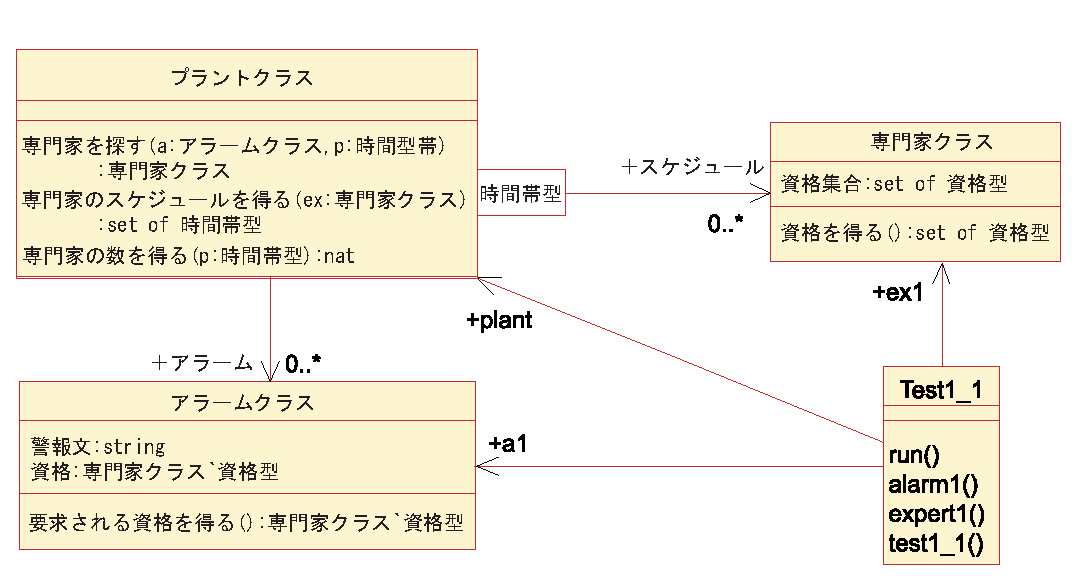
\includegraphics[width=5.967in]{fulldiagram}
\caption{UMLクラス図モデルの全体 \label{fig:fulldiagram}}
\end{center}
\end{figure}

\subsection{プラントクラス}

\begin{VDMgray}
\textbf{class} \textit{プラントクラス}

\textbf{types}
 \textbf{public} \textit{時間帯型} = \textbf{token};

\textbf{instance} \textbf{variables}
 \textit{アラーム集合} : \textbf{set} \textbf{of} \textit{アラームクラス} := \{\};
 \textit{スケジュール} : \textbf{map} \textit{時間帯型} \textbf{to} \textbf{set} \textbf{of} \textit{専門家クラス} := \{{\textbar}-\texttt{>}\};
 \textbf{inv}
   \textbf{forall} \textit{p} \textbf{in set} \textbf{dom} \textit{スケジュール} \& \textit{スケジュール}(\textit{p}) \texttt{<}\texttt{>} \{\};
 \textbf{inv}
   \textbf{forall} \textit{a} \textbf{in set} \textit{アラーム集合} \&
      \textbf{forall} \textit{p} \textbf{in set} \textbf{dom} \textit{スケジュールe} \&
         \textbf{exists} \textit{ex} \textbf{in set} \textit{スケジュール}(\textit{p}) \&
            \textit{a}.\textit{要求される資格を得る}() \textbf{in set} \textit{ex}.\textit{資格を得る}();

\textbf{operations}
 \textbf{public}
 \textit{専門家を探す} : \textit{アラームクラス} * \textit{時間帯型} ==\texttt{>} \textit{専門家クラス}
 \textit{専門家を探す}(\textit{a}, \textit{p}) ==
   \textbf{let} \textit{ex} \textbf{in set} \textit{スケジュール}(\textit{p}) \textbf{be} \textbf{st}
       \textit{a}.\textit{要求される資格を得る}() \textbf{in set} \textit{ex}.\textit{資格を得る}()
   \textbf{in} \textbf{return} \textit{ex}
 \textbf{pre} \textit{a} \textbf{in set} \textit{アラーム集合} \textbf{and}
     \textit{p} \textbf{in set} \textbf{dom} \textit{スケジュール}
 \textbf{post} \textbf{let} \textit{ex} = \textit{RESULT} \textbf{in}
       \textit{ex} \textbf{in set} \textit{スケジュール}(\textit{p}) \textbf{and}
       \textit{a}.\textit{要求される資格を得る}() \textbf{in set} \textit{ex}.\textit{資格を得る}();

 \textbf{public}
 \textit{専門家のスケジュールを得る} : \textit{専門家クラス} ==\texttt{>} \textbf{set} \textbf{of} \textit{時間帯型}
 \textit{専門家のスケジュールを得る}(\textit{ex}) ==
   \textbf{return} \{\textit{p} {\textbar} \textit{p} \textbf{in set} \textbf{dom} \textit{スケジュール} 
             \& \textit{ex} \textbf{in set} \textit{スケジュール}(\textit{p})\};

 \textbf{public}
 \textit{専門家の数を得る} : \textit{時間帯型} ==\texttt{>} \textbf{nat}
 \textit{専門家の数を得る}(\textit{p}) ==
  {\color{red} \textbf{return} \textbf{card} \textit{スケジュール} ( \textit{p} )}
  \textbf{pre} {\color{red} \textit{p} \textbf{in set} \textbf{dom} \textit{スケジュール}};
\end{VDMgray}

\begin{VDMgray}
 \textbf{public}
 \textit{スケジュールをセットする}: \textbf{map} \textit{時間帯型} \textbf{to} \textbf{set} \textbf{of} \textit{専門家クラス} ==\texttt{>} ()
 \textit{スケジュールをセットする}(\textit{sch}) ==
   \textit{スケジュール}:= \textit{sch};

 \textbf{public}
 \textit{アラームをセットする}: \textbf{set} \textbf{of} \textit{アラームクラス} ==\texttt{>} ()
 \textit{アラームをセットする}(\textit{als}) ==
   \textit{アラーム集合}:= \textit{als};

\textbf{values} -- テスト用
  \textbf{public} \textit{p1}:\textit{時間帯型} = \textbf{mk\_token}("月曜日");
  \textbf{public} \textit{p2}:\textit{時間帯型} = \textbf{mk\_token}("火曜日");
  \textbf{public} \textit{p3}:\textit{時間帯型} = \textbf{mk\_token}("水曜日");
  \textbf{public} \textit{p4}:\textit{時間帯型} = \textbf{mk\_token}("木曜日");
  \textbf{public} \textit{p5}:\textit{時間帯型} = \textbf{mk\_token}("金曜日");

\textbf{end} \textit{プラントクラス}

\end{VDMgray}


\begin{longtable}{lll}
\hline
\endhead
\hline
\endfoot
\hline
\multicolumn{1}{|p{3.086in}|}
{\raggedright
\textbf{\textit{名称}}} & 
\multicolumn{1}{p{0.660in}|}
{\raggedright
\textbf{\textit{call回数}}} & 
\multicolumn{1}{p{0.754in}|}
{\raggedright
\textbf{\textit{カバレッジ}}}
\\ \cline{1-1}\cline{2-2}\cline{3-3}
\multicolumn{1}{|p{3.086in}|}
{\raggedright
プラントクラス\`{}専門家のスケジュールを得る } & 
\multicolumn{1}{p{0.660in}|}
{\raggedright
  1 } & 
\multicolumn{1}{p{0.754in}|}
{\raggedright
100\%}
\\ \cline{1-1}\cline{2-2}\cline{3-3}
\multicolumn{1}{|p{3.086in}|}
{\raggedright
プラントクラス\`{}専門家を探す } & 
\multicolumn{1}{p{0.660in}|}
{\raggedright
  1 } & 
\multicolumn{1}{p{0.754in}|}
{\raggedright
100\%}
\\ \cline{1-1}\cline{2-2}\cline{3-3}
\multicolumn{1}{|p{3.086in}|}
{\raggedright
プラントクラス\`{}専門家の数を得る } & 
\multicolumn{1}{p{0.660in}|}
{\raggedright
  0 } & 
\multicolumn{1}{p{0.754in}|}
{\raggedright
0\%}
\\ \cline{1-1}\cline{2-2}\cline{3-3}
\multicolumn{1}{|p{3.086in}|}
{\raggedright
プラントクラス\`{}アラームをセットする } & 
\multicolumn{1}{p{0.660in}|}
{\raggedright
  1 } & 
\multicolumn{1}{p{0.754in}|}
{\raggedright
100\%}
\\ \cline{1-1}\cline{2-2}\cline{3-3}
\multicolumn{1}{|p{3.086in}|}
{\raggedright
プラントクラス\`{}スケジュールをセットする } & 
\multicolumn{1}{p{0.660in}|}
{\raggedright
  1 } & 
\multicolumn{1}{p{0.754in}|}
{\raggedright
100\%}
\\ \cline{1-1}\cline{2-2}\cline{3-3}
\multicolumn{1}{|p{3.086in}|}
{\raggedright
\textbf{\textit{合計}}} & 
\multicolumn{1}{p{0.660in}|}
{\raggedright
} & 
\multicolumn{1}{p{0.754in}|}
{\raggedright
\textbf{\textit{84\% }}} \\
\hline
\end{longtable}

\subsection{専門家クラス}

\begin{VDMgray}
\textbf{class} \textit{専門家クラス}

\textbf{types}
 \textbf{public} \textit{資格型} = \texttt{<}機械\texttt{>} {\textbar} \texttt{<}化学\texttt{>} {\textbar} \texttt{<}生物\texttt{>} {\textbar} \texttt{<}電気\texttt{>};

\textbf{instance} \textbf{variables}
 \textit{資格集合} : \textbf{set} \textbf{of} \textit{資格型};

\textbf{operations}
 \textbf{public}
 \textit{資格を得る}: () ==\texttt{>} \textbf{set} \textbf{of} \textit{資格型}
 \textit{資格を得る}() == \textbf{return} \textit{資格集合};

 \textbf{public}
 \textit{資格をセットする}: \textbf{set} \textbf{of} \textit{資格型} ==\texttt{>} ()
 \textit{資格をセットする}(\textit{qs}) ==
   \textit{資格集合}:= \textit{qs};

\textbf{end} \textit{専門家クラス}

\end{VDMgray}


\begin{longtable}{lll}
\hline
\endhead
\hline
\endfoot
\hline
\multicolumn{1}{|p{3.086in}|}
{\raggedright
\textbf{\textit{名称}}} & 
\multicolumn{1}{p{0.660in}|}
{\raggedright
\textbf{\textit{call回数}}} & 
\multicolumn{1}{p{0.754in}|}
{\raggedright
\textbf{\textit{カバレッジ}}}
\\ \cline{1-1}\cline{2-2}\cline{3-3}
\multicolumn{1}{|p{3.086in}|}
{\raggedright
専門家クラス\`{}資格を得る } & 
\multicolumn{1}{p{0.660in}|}
{\raggedright
  3 } & 
\multicolumn{1}{p{0.754in}|}
{\raggedright
100\%}
\\ \cline{1-1}\cline{2-2}\cline{3-3}
\multicolumn{1}{|p{3.086in}|}
{\raggedright
専門家クラス\`{}資格をセットする } & 
\multicolumn{1}{p{0.660in}|}
{\raggedright
  1 } & 
\multicolumn{1}{p{0.754in}|}
{\raggedright
100\%}
\\ \cline{1-1}\cline{2-2}\cline{3-3}
\multicolumn{1}{|p{3.086in}|}
{\raggedright
\textbf{\textit{合計}}} & 
\multicolumn{1}{p{0.660in}|}
{\raggedright
} & 
\multicolumn{1}{p{0.754in}|}
{\raggedright
\textbf{\textit{100\% }}}\\
\hline
\end{longtable}

\subsection{Test1クラス}


\begin{VDMgray}
\textbf{class} \textit{Test1}

\textbf{instance} \textbf{variables}
 \textit{a1} : \textit{アラームクラス};
 \textit{ex1} : \textit{専門家クラス};
 \textit{plant} : \textit{プラントクラス};

\textbf{operations}
 \textbf{public}
 \textit{run}: () ==\texttt{>} \textbf{set} \textbf{of} \textit{プラントクラス}\`{}\textit{時間帯型} * \textit{専門家クラス}
 \textit{run}() == \textit{test1}();

 \textbf{public}
 \textit{test1}: () ==\texttt{>} \textbf{set} \textbf{of} \textit{プラントクラス}\`{}\textit{時間帯型} * \textit{専門家クラス}
 \textit{test1}() ==
   (\textit{alarm1}();
    \textit{expert1}();
    \textit{plant}:= \textbf{new} \textit{プラントクラス}();
    \textit{plant}.\textit{スケジュールをセットする}(\{\textit{plant}.\textit{p1} {\textbar}-\texttt{>} \{\textit{ex1}\}\});
    \textit{plant}.\textit{アラームをセットする}(\{\textit{a1}\});
    \textbf{let} \textit{periods} = \textit{plant}.\textit{専門家のスケジュールを得る}(\textit{ex1}),
        \textit{expert} = \textit{plant}.\textit{専門家を探す}(\textit{a1},\textit{plant}.\textit{p1})
    \textbf{in}
      \textbf{return} \textbf{mk\_}(\textit{periods},\textit{expert})
  );

 \textbf{public}
 \textit{alarm1}: () ==\texttt{>} ()
 \textit{alarm1}() ==
   (\textit{a1}:= \textbf{new} \textit{アラームクラス}();
    \textit{a1}.\textit{要求資格をセットする}(\texttt{<}機械\texttt{>});
    \textit{a1}.\textit{警報文をセットする}("機械系故障"));

 \textbf{public}
 \textit{expert1}: () ==\texttt{>} ()
 \textit{expert1}() ==
   (\textit{ex1}:= \textbf{new} \textit{専門家クラス}();
    \textit{ex1}.\textit{資格をセットする}(\{\texttt{<}機械\texttt{>},\texttt{<}生物\texttt{>}\}))

\textbf{end} \textit{Test1}

\end{VDMgray}


\begin{longtable}{lll}
\hline
\endhead
\hline
\endfoot
\hline
\multicolumn{1}{|p{3.086in}|}
{\raggedright
\textbf{\textit{名称}}} & 
\multicolumn{1}{p{0.660in}|}
{\raggedright
\textbf{\textit{call回数}}} & 
\multicolumn{1}{p{0.754in}|}
{\raggedright
\textbf{\textit{カバレッジ}}}
\\ \cline{1-1}\cline{2-2}\cline{3-3}
\multicolumn{1}{|p{3.086in}|}
{\raggedright
Test1\`{}alarm1 } & 
\multicolumn{1}{p{0.660in}|}
{\raggedright
  1 } & 
\multicolumn{1}{p{0.754in}|}
{\raggedright
100\%}
\\ \cline{1-1}\cline{2-2}\cline{3-3}
\multicolumn{1}{|p{3.086in}|}
{\raggedright
Test1\`{}expert1 } & 
\multicolumn{1}{p{0.660in}|}
{\raggedright
  1 } & 
\multicolumn{1}{p{0.754in}|}
{\raggedright
100\%}
\\ \cline{1-1}\cline{2-2}\cline{3-3}
\multicolumn{1}{|p{3.086in}|}
{\raggedright
Test1`{}run } & 
\multicolumn{1}{p{0.660in}|}
{\raggedright
  1 } & 
\multicolumn{1}{p{0.754in}|}
{\raggedright
100\%}
\\ \cline{1-1}\cline{2-2}\cline{3-3}
\multicolumn{1}{|p{3.086in}|}
{\raggedright
Test1\`{}test1 } & 
\multicolumn{1}{p{0.660in}|}
{\raggedright
  1 } & 
\multicolumn{1}{p{0.754in}|}
{\raggedright
100\%}
\\ \cline{1-1}\cline{2-2}\cline{3-3}
\multicolumn{1}{|p{3.086in}|}
{\raggedright
\textbf{\textit{合計}}} & 
\multicolumn{1}{p{0.660in}|}
{\raggedright
} & 
\multicolumn{1}{p{0.754in}|}
{\raggedright
\textbf{\textit{100\% }}}\\
\hline
\end{longtable}

  

\end{document}
